\documentclass{beamer}
\mode<presentation>
\usepackage{amsmath}
\usepackage{amssymb}
%\usepackage{advdate}
\usepackage{adjustbox}
\usepackage{subcaption}
\usepackage{enumitem}
\usepackage{multicol}
\usepackage{mathtools}
\usepackage{listings}
\usepackage{url}
\def\UrlBreaks{\do\/\do-}
\usetheme{Boadilla}
\usecolortheme{lily}
\setbeamertemplate{footline}
{
  \leavevmode%
  \hbox{%
  \begin{beamercolorbox}[wd=\paperwidth,ht=2.25ex,dp=1ex,right]{author in head/foot}%
    \insertframenumber{} / \inserttotalframenumber\hspace*{2ex} 
  \end{beamercolorbox}}%
  \vskip0pt%
}

\providecommand{\nCr}[2]{\,^{#1}C_{#2}} % nCr
\providecommand{\nPr}[2]{\,^{#1}P_{#2}} % nPr
\providecommand{\mbf}{\mathbf}
\providecommand{\pr}[1]{\ensuremath{\Pr\left(#1\right)}}
\providecommand{\qfunc}[1]{\ensuremath{Q\left(#1\right)}}
\providecommand{\sbrak}[1]{\ensuremath{{}\left[#1\right]}}
\providecommand{\lsbrak}[1]{\ensuremath{{}\left[#1\right.}}
\providecommand{\rsbrak}[1]{\ensuremath{{}\left.#1\right]}}
\providecommand{\brak}[1]{\ensuremath{\left(#1\right)}}
\providecommand{\lbrak}[1]{\ensuremath{\left(#1\right.}}
\providecommand{\rbrak}[1]{\ensuremath{\left.#1\right)}}
\providecommand{\cbrak}[1]{\ensuremath{\left\{#1\right\}}}
\providecommand{\lcbrak}[1]{\ensuremath{\left\{#1\right.}}
\providecommand{\rcbrak}[1]{\ensuremath{\left.#1\right\}}}
\theoremstyle{remark}
\newtheorem{rem}{Remark}
\newcommand{\sgn}{\mathop{\mathrm{sgn}}}
\providecommand{\abs}[1]{\left\vert#1\right\vert}
\providecommand{\res}[1]{\Res\displaylimits_{#1}} 
\providecommand{\norm}[1]{\lVert#1\rVert}
\providecommand{\mtx}[1]{\mathbf{#1}}
\providecommand{\mean}[1]{E\left[ #1 \right]}
\providecommand{\fourier}{\overset{\mathcal{F}}{ \rightleftharpoons}}
%\providecommand{\hilbert}{\overset{\mathcal{H}}{ \rightleftharpoons}}
\providecommand{\system}{\overset{\mathcal{H}}{ \longleftrightarrow}}
	%\newcommand{\solution}[2]{\textbf{Solution:}{#1}}
%\newcommand{\solution}{\noindent \textbf{Solution: }}
\providecommand{\dec}[2]{\ensuremath{\overset{#1}{\underset{#2}{\gtrless}}}}
\newcommand{\myvec}[1]{\ensuremath{\begin{pmatrix}#1\end{pmatrix}}}
\let\vec\mathbf

\lstset{
%language=C,
frame=single, 
breaklines=true,
columns=fullflexible
}

\numberwithin{equation}{section}

\lstset{
  language=Python,
  basicstyle=\ttfamily\small,
  keywordstyle=\color{blue},
  stringstyle=\color{orange},
  numbers=left,
  numberstyle=\tiny\color{gray},
  breaklines=true,
  showstringspaces=false
}

\title{Problem 1.5.6}
\author{Darisy Sreetej}

\date{\today} 
\begin{document}

\begin{frame}
\titlepage
\end{frame}

\section*{Outline}
\begin{frame}
\tableofcontents
\end{frame}
\section{Problem}
\begin{frame}
\frametitle{Problem Statement}
%
 The point which divides the line segment joining the points $\brak{7,-6}$ and $\brak{3, 4}$ in the ratio $1 : 2$ is \dots.
 \begin{table}[h!]    
  \centering
  

  \caption{Variables given}
  \label{tab 1.4.9.2}
\end{table}
\end{frame}

%\subsection{Literature}
\section{Solution}
\subsection{Section Formula}
\begin{frame}
\frametitle{Section Formula}
%\framesubtitle{Literature}
Formula:
\begin{align}
\vec{P}=\frac{k(\vec{B})+(\vec{A})}{k+1}
\end{align}
Where: 

\centering{'k' is the ratio in which the point divides the line segment}

\begin{align}
\vec{A}=\myvec{7\\-6} \hspace{1cm} \vec{B}=\myvec{3\\4} 
\end{align}

\end{frame}
\subsection{Obtaining $k$ Value}
\begin{frame}
\frametitle{Obtaining $k$ Value}
According to the problem , 
The point $\vec{P}$ divides the line segment joining $\vec{A}$ and $\vec{B}$ in the ratio $1:2$

\centering{Hence , k=2}
\end{frame}
\subsection{Obtaining Point}
\begin{frame}
\frametitle{Obtaining Point}

\begin{align}
\vec{P}=\frac{2\vec{B}+\vec{A}}{3}&=\frac{2\myvec{7\\-6}+\myvec{3\\4}}{3}=\frac{\myvec{17\\-8}}{3} \\
\vec{P}
&=\myvec{\frac{17}{3}\\\frac{-8}{3}}
\end{align}

Hence the coordinates of $\vec{P}$ are $\brak{\frac{17}{3},\frac{-8}{3}}$


\end{frame}

\subsection{Plot}
\begin{frame}[fragile]
\frametitle{Plot}

\begin{figure}[h!]
   \centering
   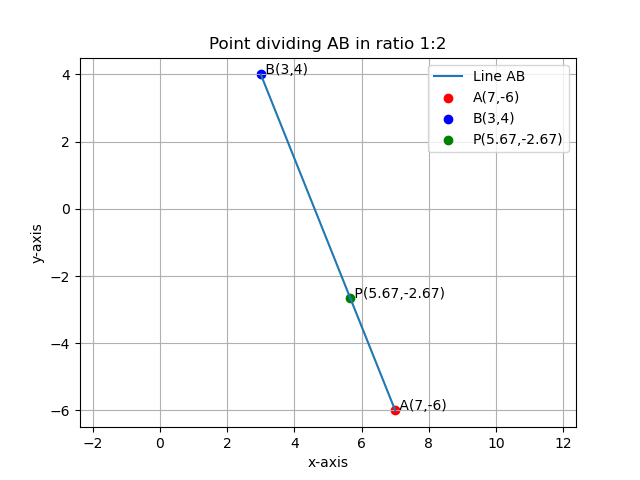
\includegraphics[width=0.9\linewidth]{figs/plot.png}
	\caption{}
   \label{stemplot}
\end{figure}
\end{frame}

\section{C Code}

\begin{frame}[fragile]
\frametitle{C Code for generating points on line}
\begin{lstlisting}[language=C]
   #include <stdio.h>

//Store the given values as global constants
const int Ax = 7, Ay = -6;
 const int bx = 3 , By =4 ;
 const int m =1,n=2;

 // Function to compute the dividing point 
 void get_dividing_point(float *Px, float *Py)
 {
 *Px=(n*Ax + m*Bx)/(float)(m+n);
 *Py=(n*Ay + m*By)/(float)(m+n);
 }

 //Function to print stored values 

\end{lstlisting}
\end{frame}

\begin{frame}[fragile]
\frametitle{C Code for generating points on line}
\begin{lstlisting}[language=C]
        void print_values()
 {
 printf("Point A = (%d,%d)\n",Ax,Ay);
printf("Point B = (%d,%d)\n",Bx,By);
printf("Ratio m;n = %d:%d\n",m,n);
 }
\end{lstlisting}
\end{frame}

\section{Python Code}
\begin{frame}[fragile]
\frametitle{Python Code for Plotting}
\begin{lstlisting}[language=Python]
import sys
import math
sys.path.insert(0, '/home/darisy-sreetej/Downloads/codes/CoordGeo')

import numpy as np
import numpy.linalg as LA
import matplotlib.pyplot as plt
import matplotlib.image as mpimg

# local imports
from line.funcs import *
from triangle.funcs import *

# Points A and B
A = np.array([7, -6])
B = np.array([3, 4])



\end{lstlisting}
\end{frame}

\begin{frame}[fragile]
\frametitle{Python Code for Plotting}
\begin{lstlisting}[language=Python]
# Ratio m:n = 1:2
m, n = 1, 2

# Section formula in vector form: P = (nA + mB) / (m+n)
P = (n*A + m*B) / (m+n)

# Generate line coordinates for plotting
line_AB = line_gen(A, B)

# Plotting
plt.plot(line_AB[0,:], line_AB[1,:], label="Line AB")  # Line AB
plt.scatter(A[0], A[1], color='red', label='A(7,-6)')
plt.scatter(B[0], B[1], color='blue', label='B(3,4)')
plt.scatter(P[0], P[1], color='green', label=f'P({P[0]:.2f},{P[1]:.2f})')

# Add text labels
plt.text(A[0], A[1], ' A(7,-6)', fontsize=10)

\end{lstlisting}
\end{frame}

\begin{frame}[fragile]
\frametitle{Python Code for Plotting}
\begin{lstlisting}[language=Python]
plt.text(B[0], B[1], ' B(3,4)', fontsize=10)
plt.text(P[0], P[1], f' P({P[0]:.2f},{P[1]:.2f})', fontsize=10)

# Formatting
plt.xlabel('x-axis')
plt.ylabel('y-axis')
plt.legend()
plt.grid(True)
plt.axis('equal')
plt.title("Point dividing AB in ratio 1:2")
plt.savefig("../figs/plot.png")
plt.show()

\end{lstlisting}
\end{frame}

\end{document}